\chapter{Théorie des couleurs}

\noindent
\textit{Dans le chapitre précédent, nous avons étudié les principes fondamentaux de la composition graphique. Nous avons vu comment organiser les éléments visuels dans un espace donné, en respectant l'équilibre, la hiérarchie, l'alignement, le contraste, la proximité, la répétition et l'espace négatif. Parmi les éléments du langage visuel, nous avons mentionné la couleur, mais sans entrer dans le détail. C'est l'objet de ce chapitre.}

\vspace{1em}

\noindent
La couleur est bien plus qu'un simple attribut esthétique : c'est un \terme{outil de communication} puissant. Elle attire l'attention, hiérarchise l'information, suscite des émotions, transmet des significations, structure la composition. Un designer qui ne maîtrise pas la couleur passe à côté d'un des leviers les plus importants de son métier.

\vspace{1em}

\noindent
Dans ce chapitre, nous allons étudier la couleur sous tous ses aspects : sa définition, sa perception, ses systèmes d'organisation, ses harmonies, sa psychologie, sa mise en œuvre technique. Nous verrons comment construire une palette de couleurs cohérente, comment utiliser la couleur pour transmettre un message, et comment éviter les erreurs les plus fréquentes. À la fin de ce chapitre, tu disposeras des connaissances théoriques et des méthodes pratiques nécessaires pour utiliser la couleur de manière professionnelle.

% ============================================================
\section{Définition et rôle de la couleur en design graphique}
% ============================================================

\subsection{Qu'est-ce que la couleur ?}

\begin{quote}
\textbf{La couleur est la sensation visuelle produite par la lumière réfléchie ou émise par un objet, perçue par l'œil et interprétée par le cerveau.}
\end{quote}

Cette définition, en apparence simple, mérite d'être décomposée.

\subsubsection{Une sensation, pas une propriété}

La couleur n'est pas une propriété intrinsèque des objets : c'est une \terme{sensation}. Un objet n'est pas « rouge » en lui-même : il \emph{réfléchit} certaines longueurs d'onde de la lumière, que notre œil perçoit comme du rouge. Si l'éclairage change, la couleur perçue change aussi. C'est pourquoi la couleur est une expérience \terme{subjective} et \terme{contextuelle}.

\subsubsection{Une interprétation du cerveau}

La perception de la couleur ne dépend pas seulement de l'œil, mais aussi du cerveau. Celui-ci interprète les signaux nerveux en fonction du contexte, de la mémoire, de la culture. Deux personnes peuvent voir la même couleur et la nommer différemment. De même, une couleur peut paraître différente selon les couleurs qui l'entourent (c'est le \terme{contraste simultané}).

\subsubsection{Une longueur d'onde}

Physiquement, la lumière est une onde électromagnétique. Les longueurs d'onde visibles par l'œil humain s'étendent d'environ 380 nanomètres (violet) à 780 nanomètres (rouge). Chaque longueur d'onde correspond à une couleur du spectre.

\subsection{Les trois dimensions de la couleur}

Toute couleur peut être décrite selon trois dimensions :

\begin{enumerate}[label=\textbf{\arabic*.}]
    \item \terme{La teinte} (ou \emph{hue}) : c'est la couleur elle-même (rouge, bleu, vert, jaune, etc.). Elle correspond à la longueur d'onde dominante.
    \item \terme{La saturation} (ou \emph{chroma}) : c'est l'intensité de la couleur. Une couleur très saturée est vive, pure ; une couleur peu saturée est terne, grisée.
    \item \terme{La luminosité} (ou \emph{valeur}) : c'est la clarté ou l'obscurité de la couleur. Une couleur claire est proche du blanc ; une couleur sombre est proche du noir.
\end{enumerate}

Ces trois dimensions sont représentées dans de nombreux systèmes colorimétriques (TSL, TSL, HSV, etc.). Nous y reviendrons dans la section 10.

\subsection{Le rôle de la couleur en design graphique}

La couleur remplit plusieurs fonctions essentielles en design graphique.

\subsubsection{Fonction d'attention}

La couleur \terme{attire l'attention}. Une couleur vive sur un fond neutre se remarque immédiatement. C'est pourquoi la couleur est souvent utilisée pour mettre en valeur un élément important : un bouton d'appel à l'action, un titre, un logo.

\subsubsection{Fonction de hiérarchie}

La couleur \terme{hiérarchise l'information}. En utilisant des couleurs différentes pour des niveaux d'information différents, on guide le regard du spectateur. Par exemple, un titre en rouge, un sous-titre en noir, un texte en gris.

\subsubsection{Fonction d'identification}

La couleur \terme{identifie} une marque, un produit, un service. Pense à Coca-Cola (rouge), à Facebook (bleu), à Starbucks (vert). La couleur est un élément clé de l'identité visuelle.

\subsubsection{Fonction d'émotion}

La couleur \terme{émeut}. Elle suscite des réactions affectives : joie, tristesse, calme, excitation, peur, désir. La psychologie des couleurs étudie ces effets (voir section 8).

\subsubsection{Fonction de signification}

La couleur \terme{signifie}. Elle porte des significations culturelles : le rouge pour le danger ou l'amour, le vert pour la nature ou l'espoir, le noir pour le deuil ou l'élégance. Ces significations varient selon les cultures (voir section 8).

\subsubsection{Fonction d'organisation}

La couleur \terme{organise} la composition. Elle délimite des zones, crée des groupes, structure l'espace. Par exemple, un fond de couleur différente pour une zone d'information.

\subsection{Couleur et composition}

La couleur est indissociable de la composition. Elle interagit avec les autres éléments :

\begin{itemize}
    \item Avec la \terme{forme} : une même forme dans une couleur différente n'a pas le même impact.
    \item Avec la \terme{typographie} : la couleur du texte doit contraster avec le fond pour être lisible.
    \item Avec l'\terme{image} : la couleur de l'image doit s'harmoniser avec le reste de la composition.
    \item Avec l'\terme{espace négatif} : la couleur du fond influence la perception des éléments.
\end{itemize}

\subsection*{Conclusion de la section}

\begin{retenir}
La couleur est une \terme{sensation} produite par la lumière, perçue par l'œil et interprétée par le cerveau. Elle se décrit selon trois dimensions : la \terme{teinte}, la \terme{saturation} et la \terme{luminosité}. En design graphique, elle remplit des fonctions d'\terme{attention}, de \terme{hiérarchie}, d'\terme{identification}, d'\terme{émotion}, de \terme{signification} et d'\terme{organisation}. Elle est indissociable de la composition.
\end{retenir}

Maintenant que nous avons défini la couleur, nous allons, dans la section suivante, étudier le \terme{cercle chromatique}, qui est l'outil fondamental pour organiser et comprendre les relations entre les couleurs.

% ============================================================
\section{Le cercle chromatique}
% ============================================================

\subsection{Qu'est-ce que le cercle chromatique ?}

\begin{quote}
\textbf{Le cercle chromatique est une représentation circulaire des couleurs, organisée selon leurs relations. Il permet de visualiser les couleurs primaires, secondaires et tertiaires, ainsi que les relations entre elles (complémentarité, analogie, etc.).}
\end{quote}

Le cercle chromatique est un outil pédagogique et pratique. Il aide à comprendre les relations entre les couleurs et à construire des harmonies.

\subsection{Historique}

Le premier cercle chromatique est attribué à \terme{Isaac Newton} (1704), qui a disposé les couleurs du spectre sur un cercle. Par la suite, de nombreux artistes et scientifiques ont proposé leurs propres versions : Goethe, Chevreul, Itten, Munsell, etc.

Le cercle chromatique le plus utilisé aujourd'hui en design graphique est basé sur le modèle \terme{RVB} (rouge, vert, bleu) pour l'écran et \terme{CMJN} (cyan, magenta, jaune, noir) pour l'impression. Mais le cercle traditionnel des artistes est basé sur le modèle \terme{RJB} (rouge, jaune, bleu).

\subsection{Les couleurs primaires}

Les \terme{couleurs primaires} sont les couleurs de base, qui ne peuvent pas être obtenues par mélange. Selon le modèle utilisé, les primaires diffèrent :

\begin{itemize}
    \item \terme{Modèle RJB} (artiste) : rouge, jaune, bleu.
    \item \terme{Modèle RVB} (écran) : rouge, vert, bleu.
    \item \terme{Modèle CMJN} (impression) : cyan, magenta, jaune.
\end{itemize}

Dans ce chapitre, nous utiliserons principalement le modèle \terme{RVB} pour l'écran et le modèle \terme{CMJN} pour l'impression, car ce sont ceux utilisés en design graphique numérique.

\subsection{Les couleurs secondaires}

Les \terme{couleurs secondaires} sont obtenues par le mélange de deux couleurs primaires :

\begin{itemize}
    \item Rouge + Vert = Jaune (en RVB).
    \item Rouge + Bleu = Magenta (en RVB).
    \item Vert + Bleu = Cyan (en RVB).
\end{itemize}

En synthèse soustractive (CMJN) :

\begin{itemize}
    \item Cyan + Magenta = Bleu.
    \item Cyan + Jaune = Vert.
    \item Magenta + Jaune = Rouge.
\end{itemize}

\subsection{Les couleurs tertiaires}

Les \terme{couleurs tertiaires} sont obtenues par le mélange d'une couleur primaire et d'une couleur secondaire :

\begin{itemize}
    \item Rouge-orange, jaune-orange, jaune-vert, bleu-vert, bleu-violet, rouge-violet.
\end{itemize}

\subsection{L'organisation du cercle}

Le cercle chromatique est organisé de manière à ce que les couleurs voisines soient proches et les couleurs opposées soient complémentaires. Il comporte généralement 12 couleurs (3 primaires, 3 secondaires, 6 tertiaires), mais peut être étendu à 24, 48, etc.

\begin{figure}[ht]
\centering
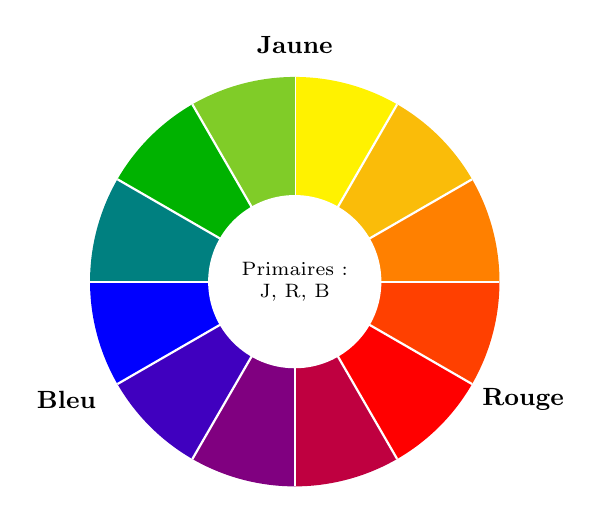
\begin{tikzpicture}
\foreach \i/\c in {0/yellow,1/yellow!50!orange,2/orange,3/orange!50!red,4/red,5/red!50!violet,6/violet,7/blue!50!violet,8/blue,9/blue!50!green,10/green!70!black,11/yellow!50!green}{
  \fill[\c] (0,0) -- ({90-\i*30}:2.6) arc({90-\i*30}:{60-\i*30}:2.6) -- cycle;
  \draw[white,thick] (0,0) -- ({90-\i*30}:2.6);}
\fill[white] (0,0) circle(1.1);
\node[font=\scriptsize,align=center] at (0,0) {Primaires :\\J, R, B};
\node[font=\small\bfseries] at (0,3) {Jaune};
\node[font=\small\bfseries] at (2.9,-1.5) {Rouge};
\node[font=\small\bfseries] at (-2.9,-1.5) {Bleu};
\end{tikzpicture}
\caption{Cercle chromatique à 12 couleurs (modèle artistique) : les couleurs opposées sont complémentaires.}
\end{figure}

\subsection{Les relations entre couleurs}

Le cercle chromatique permet de visualiser plusieurs relations :

\begin{itemize}
    \item \terme{Couleurs complémentaires} : opposées sur le cercle (rouge/vert, bleu/orange, jaune/violet).
    \item \terme{Couleurs analogues} : voisines sur le cercle (bleu, bleu-vert, vert).
    \item \terme{Couleurs triadiques} : formant un triangle équilatéral sur le cercle.
    \item \terme{Couleurs tétradiques} : formant un carré ou un rectangle sur le cercle.
\end{itemize}

Ces relations sont à la base des harmonies chromatiques (voir section 6).

\subsection*{Conclusion de la section}

\begin{retenir}
Le \terme{cercle chromatique} est une représentation circulaire des couleurs qui permet de visualiser leurs relations. Il distingue les couleurs \terme{primaires} (rouge, vert, bleu en RVB ; cyan, magenta, jaune en CMJN), les couleurs \terme{secondaires} (mélange de deux primaires) et les couleurs \terme{tertiaires} (mélange d'une primaire et d'une secondaire). Il permet d'identifier les relations de \terme{complémentarité}, d'\terme{analogie}, de \terme{triade} et de \terme{tétrade}.
\end{retenir}

Maintenant que nous connaissons le cercle chromatique, nous allons, dans la section suivante, étudier plus en détail les \terme{couleurs primaires, secondaires et tertiaires}, ainsi que leurs propriétés.

% ============================================================
\section{Les couleurs primaires, secondaires et tertiaires}
% ============================================================

\subsection{Les couleurs primaires}

\subsubsection{Définition}

Les \terme{couleurs primaires} sont les couleurs de base qui ne peuvent pas être obtenues par mélange d'autres couleurs. Elles sont à l'origine de toutes les autres couleurs.

\subsubsection{Les primaires en synthèse additive (RVB)}

En synthèse \terme{additive}, utilisée pour les écrans, les primaires sont :

\begin{itemize}
    \item \terme{Rouge} (\emph{Red})
    \item \terme{Vert} (\emph{Green})
    \item \terme{Bleu} (\emph{Blue})
\end{itemize}

Le mélange des trois primaires donne du blanc. C'est le modèle \terme{RVB}, utilisé par tous les écrans (ordinateurs, téléphones, télévisions).

\subsubsection{Les primaires en synthèse soustractive (CMJN)}

En synthèse \terme{soustractive}, utilisée pour l'impression, les primaires sont :

\begin{itemize}
    \item \terme{Cyan}
    \item \terme{Magenta}
    \item \terme{Jaune} (\emph{Yellow})
\end{itemize}

Le mélange des trois primaires donne du noir (en théorie). En pratique, on ajoute du \terme{noir} (\emph{Key}) pour obtenir un noir profond : c'est le modèle \terme{CMJN}.

\subsubsection{Les primaires en modèle artistique (RJB)}

Dans le modèle traditionnel des artistes (peinture), les primaires sont :

\begin{itemize}
    \item \terme{Rouge}
    \item \terme{Jaune}
    \item \terme{Bleu}
\end{itemize}

Ce modèle est encore utilisé en pédagogie artistique, mais il est moins précis que les modèles RVB et CMJN.

\subsection{Les couleurs secondaires}

\subsubsection{Définition}

Les \terme{couleurs secondaires} sont obtenues par le mélange de deux couleurs primaires.

\subsubsection{En RVB}

\begin{itemize}
    \item Rouge + Vert = \terme{Jaune}
    \item Rouge + Bleu = \terme{Magenta}
    \item Vert + Bleu = \terme{Cyan}
\end{itemize}

\subsubsection{En CMJN}

\begin{itemize}
    \item Cyan + Magenta = \terme{Bleu}
    \item Cyan + Jaune = \terme{Vert}
    \item Magenta + Jaune = \terme{Rouge}
\end{itemize}

\subsection{Les couleurs tertiaires}

\subsubsection{Définition}

Les \terme{couleurs tertiaires} sont obtenues par le mélange d'une couleur primaire et d'une couleur secondaire.

\subsubsection{Liste}

\begin{itemize}
    \item Rouge-orange (rouge + orange)
    \item Jaune-orange (jaune + orange)
    \item Jaune-vert (jaune + vert)
    \item Bleu-vert (bleu + vert)
    \item Bleu-violet (bleu + violet)
    \item Rouge-violet (rouge + violet)
\end{itemize}

\subsection{Tableau récapitulatif}

\begin{table}[h!]
\centering
\begin{tabular}{@{}lll@{}}
\toprule
\textbf{Type} & \textbf{Modèle RVB} & \textbf{Modèle CMJN} \\
\midrule
Primaires & Rouge, Vert, Bleu & Cyan, Magenta, Jaune \\
Secondaires & Jaune, Magenta, Cyan & Bleu, Vert, Rouge \\
Tertiaires & Rouge-orange, etc. & Cyan-vert, etc. \\
\bottomrule
\end{tabular}
\caption{Les couleurs primaires, secondaires et tertiaires selon le modèle.}
\end{table}

\subsection*{Conclusion de la section}

\begin{retenir}
Les couleurs \terme{primaires} sont les couleurs de base (RVB pour l'écran, CMJN pour l'impression). Les couleurs \terme{secondaires} sont obtenues par le mélange de deux primaires. Les couleurs \terme{tertiaires} sont obtenues par le mélange d'une primaire et d'une secondaire. Cette classification est fondamentale pour comprendre les harmonies chromatiques.
\end{retenir}

Maintenant que nous connaissons les différentes catégories de couleurs, nous allons, dans la section suivante, étudier la distinction entre \terme{couleurs chaudes et couleurs froides}, qui joue un rôle important dans la perception et l'émotion.

% ============================================================
\section{Les couleurs chaudes et froides}
% ============================================================

\subsection{Qu'est-ce qu'une couleur chaude ou froide ?}

\begin{quote}
\textbf{Les couleurs chaudes sont celles qui évoquent la chaleur (rouge, orange, jaune). Les couleurs froides sont celles qui évoquent le froid (bleu, vert, violet).}
\end{quote}

Cette distinction est \terme{perceptive} et \terme{culturelle}. Elle repose sur des associations d'idées : le feu, le soleil, l'été pour les couleurs chaudes ; l'eau, la glace, l'hiver pour les couleurs froides.

\subsection{Le cercle chromatique et la température}

Sur le cercle chromatique, on peut distinguer deux moitiés :

\begin{itemize}
    \item \terme{Moitié chaude} : du rouge au jaune-vert, en passant par l'orange.
    \item \terme{Moitié froide} : du vert au rouge-violet, en passant par le bleu.
\end{itemize}

Certaines couleurs sont \terme{ambivalentes} : le vert peut être chaud (vert-jaune) ou froid (vert-bleu). Le violet peut être chaud (violet-rouge) ou froid (violet-bleu).

\subsection{Effets des couleurs chaudes et froides}

\subsubsection{Effet de température}

Les couleurs chaudes \terme{réchauffent} une composition ; les couleurs froides la \terme{refroidissent}. Ce effet est utilisé en design pour créer des ambiances.

\subsubsection{Effet de profondeur}

Les couleurs chaudes \terme{avancent} (elles semblent plus proches) ; les couleurs froides \terme{reculent} (elles semblent plus éloignées). Ce effet est utilisé pour créer de la profondeur.

\subsubsection{Effet d'émotion}

Les couleurs chaudes évoquent l'\terme{énergie}, la \terme{passion}, l'\terme{urgence}, la \terme{joie}. Les couleurs froides évoquent le \terme{calme}, la \terme{sérénité}, la \terme{tristesse}, la \terme{rigueur}.

\subsubsection{Effet de contraste}

Le contraste entre chaud et froid est un contraste puissant. Il attire l'attention et crée de la tension.

\subsection{Applications en design}

\begin{itemize}
    \item \terme{Publicité alimentaire} : couleurs chaudes (rouge, orange) pour stimuler l'appétit.
    \item \terme{Publicité de produits frais} : couleurs froides (bleu, vert) pour évoquer la fraîcheur.
    \item \terme{Identité de marque} : couleurs chaudes pour une marque dynamique, couleurs froides pour une marque sérieuse.
    \item \terme{Interfaces} : couleurs chaudes pour les appels à l'action, couleurs froides pour les fonds.
\end{itemize}

\subsection*{Conclusion de la section}

\begin{retenir}
Les \terme{couleurs chaudes} (rouge, orange, jaune) évoquent la chaleur, l'énergie, la passion. Les \terme{couleurs froides} (bleu, vert, violet) évoquent le froid, le calme, la sérénité. Cette distinction joue sur la température perçue, la profondeur, l'émotion et le contraste. Elle est utilisée en design pour créer des ambiances et transmettre des messages.
\end{retenir}

Maintenant que nous avons étudié la température des couleurs, nous allons, dans la section suivante, approfondir les trois dimensions de la couleur : la \terme{teinte}, la \terme{saturation} et la \terme{luminosité}.

% ============================================================
% ============================================================
\section{La teinte, la saturation et la luminosité}
% ============================================================

\subsection{Les trois dimensions de la couleur}

Toute couleur peut être décrite selon trois dimensions :

\begin{enumerate}[label=\textbf{\arabic*.}]
    \item \terme{La teinte} (\emph{hue}) : la couleur elle-même.
    \item \terme{La saturation} (\emph{saturation}) : l'intensité de la couleur.
    \item \terme{La luminosité} (\emph{value} ou \emph{brightness}) : la clarté de la couleur.
\end{enumerate}

\subsection{La teinte}

\subsubsection{Définition}

La \terme{teinte} est la qualité qui distingue une couleur d'une autre : rouge, bleu, vert, jaune, etc. Elle correspond à la longueur d'onde dominante de la lumière.

\subsubsection{Représentation}

Sur le cercle chromatique, la teinte est représentée par un angle (0° à 360°). Dans les logiciels, elle est souvent représentée par un cercle chromatique ou un curseur.

\subsubsection{Teintes et nuances}

On distingue :

\begin{itemize}
    \item Les \terme{teintes pures} : couleurs saturées du cercle chromatique.
    \item Les \terme{nuances} : mélanges avec du blanc, du noir ou du gris.
\end{itemize}

\subsection{La saturation}

\subsubsection{Définition}

La \terme{saturation} est l'intensité de la couleur. Une couleur très saturée est \terme{vive}, \terme{pure}. Une couleur peu saturée est \terme{terne}, \terme{grisée}.

\subsubsection{Représentation}

La saturation est représentée par un pourcentage (0\% à 100\%). À 0\%, la couleur est un gris. À 100\%, la couleur est pure.

\subsubsection{Effets de la saturation}

\begin{itemize}
    \item \terme{Saturation élevée} : attention, énergie, intensité.
    \item \terme{Saturation faible} : calme, élégance, discrétion.
\end{itemize}

\subsection{La luminosité}

\subsubsection{Définition}

La \terme{luminosité} est la clarté ou l'obscurité de la couleur. Une couleur claire est proche du blanc ; une couleur sombre est proche du noir.

\subsubsection{Représentation}

La luminosité est représentée par un pourcentage (0\% à 100\%). À 0\%, la couleur est noire. À 100\%, la couleur est blanche.

\subsubsection{Effets de la luminosité}

\begin{itemize}
    \item \terme{Luminosité élevée} : légèreté, douceur, ouverture.
    \item \terme{Luminosité faible} : poids, sérieux, mystère.
\end{itemize}

\subsection{Les modèles colorimétriques}

Les trois dimensions sont utilisées dans différents modèles :

\begin{itemize}
    \item \terme{TSL} (Teinte, Saturation, Luminosité).
    \item \terme{HSV} (Hue, Saturation, Value).
    \item \terme{HSL} (Hue, Saturation, Lightness).
\end{itemize}

Ces modèles sont utilisés dans les logiciels de design.

\subsection{Applications pratiques}

\begin{itemize}
    \item \terme{Créer une palette} : choisir une teinte, puis varier la saturation et la luminosité.
    \item \terme{Créer du contraste} : jouer sur la luminosité.
    \item \terme{Créer une ambiance} : jouer sur la saturation.
    \item \terme{Hiérarchiser} : utiliser des couleurs plus ou moins saturées.
\end{itemize}

\subsection*{Conclusion de la section}

\begin{retenir}
Toute couleur se décrit selon trois dimensions : la \terme{teinte} (la couleur elle-même), la \terme{saturation} (l'intensité) et la \terme{luminosité} (la clarté). Ces trois dimensions permettent de créer des variations infinies à partir d'une même teinte. Elles sont à la base des harmonies chromatiques et des palettes de couleurs.
\end{retenir}

Maintenant que nous maîtrisons les trois dimensions de la couleur, nous allons, dans la section suivante, étudier les \terme{harmonies chromatiques}, c'est-à-dire les combinaisons de couleurs qui fonctionnent bien ensemble.

% ============================================================
\section{Les harmonies chromatiques}
% ============================================================

\subsection{Qu'est-ce qu'une harmonie chromatique ?}

\begin{quote}
\textbf{Une harmonie chromatique est une combinaison de couleurs qui produit un effet agréable et cohérent. Elle repose sur des relations entre les couleurs, définies à partir du cercle chromatique.}
\end{quote}

Une harmonie n'est pas une règle absolue : elle dépend du contexte, du message, du public. Mais elle fournit des repères utiles pour construire une palette.

\subsection{Les principales harmonies}

\subsubsection{Harmonie monochromatique}

Une seule teinte, déclinée en différentes saturations et luminosités.

\begin{itemize}
    \item \terme{Avantages} : cohérence, simplicité, élégance.
    \item \terme{Inconvénients} : monotonie, manque de contraste.
    \item \terme{Exemples} : une composition en bleu (bleu clair, bleu moyen, bleu foncé).
\end{itemize}

\subsubsection{Harmonie analogue}

Des teintes voisines sur le cercle chromatique.

\begin{itemize}
    \item \terme{Avantages} : douceur, cohérence, naturel.
    \item \terme{Inconvénients} : manque de contraste, peu d'impact.
    \item \terme{Exemples} : bleu, bleu-vert, vert.
\end{itemize}

\subsubsection{Harmonie complémentaire}

Deux teintes opposées sur le cercle chromatique.

\begin{itemize}
    \item \terme{Avantages} : contraste fort, impact, dynamisme.
    \item \terme{Inconvénients} : tension, fatigue visuelle si mal utilisée.
    \item \terme{Exemples} : rouge et vert, bleu et orange, jaune et violet.
\end{itemize}

\subsubsection{Harmonie complémentaire divisée}

Une teinte et les deux teintes voisines de sa complémentaire.

\begin{itemize}
    \item \terme{Avantages} : contraste moins brutal que la complémentaire, richesse.
    \item \terme{Inconvénients} : plus complexe à équilibrer.
    \item \terme{Exemples} : bleu, rouge-orange, jaune-orange.
\end{itemize}

\subsubsection{Harmonie triadique}

Trois teintes formant un triangle équilatéral sur le cercle chromatique.

\begin{itemize}
    \item \terme{Avantages} : équilibre, richesse, dynamisme.
    \item \terme{Inconvénients} : difficile à équilibrer.
    \item \terme{Exemples} : rouge, jaune, bleu.
\end{itemize}

\subsubsection{Harmonie tétradique}

Quatre teintes formant un carré ou un rectangle sur le cercle chromatique.

\begin{itemize}
    \item \terme{Avantages} : richesse, variété.
    \item \terme{Inconvénients} : difficile à équilibrer, risque de confusion.
    \item \terme{Exemples} : rouge, jaune, vert, bleu.
\end{itemize}

\begin{figure}[ht]
\centering
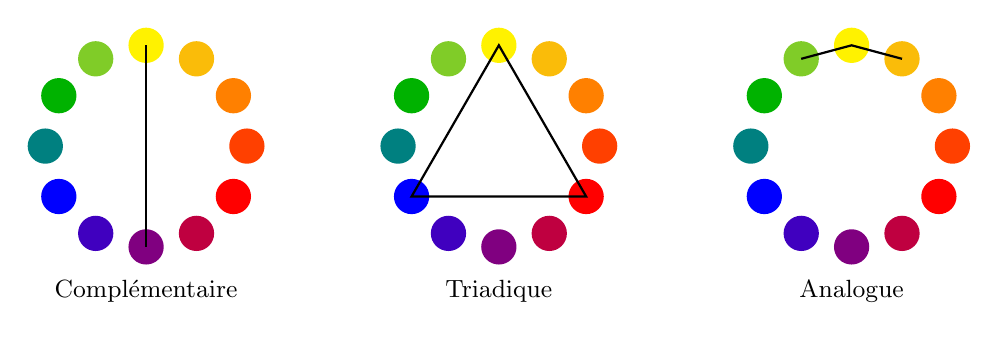
\begin{tikzpicture}[scale=0.8]
\foreach \s/\lab in {0/Complémentaire,5.6/Triadique,11.2/Analogue}{
  \foreach \i/\c in {0/yellow,1/yellow!50!orange,2/orange,3/orange!50!red,4/red,5/red!50!violet,6/violet,7/blue!50!violet,8/blue,9/blue!50!green,10/green!70!black,11/yellow!50!green}{
    \fill[\c] ({\s+1.6*sin(\i*30)},{1.6*cos(\i*30)}) circle(0.28);}
  \node[font=\small] at (\s,-2.3) {\lab};}
\draw[thick] ({0+1.6*sin(0)},{1.6*cos(0)}) -- ({0+1.6*sin(180)},{1.6*cos(180)});
\draw[thick] ({5.6+1.6*sin(0)},{1.6*cos(0)}) -- ({5.6+1.6*sin(120)},{1.6*cos(120)}) -- ({5.6+1.6*sin(240)},{1.6*cos(240)}) -- cycle;
\draw[thick] ({11.2+1.6*sin(-30)},{1.6*cos(-30)}) -- ({11.2+1.6*sin(0)},{1.6*cos(0)}) -- ({11.2+1.6*sin(30)},{1.6*cos(30)});
\end{tikzpicture}
\caption{Trois harmonies repérées sur le cercle chromatique : une droite (complémentaire), un triangle équilatéral (triadique) et trois teintes voisines (analogue).}
\end{figure}

\subsection{Tableau récapitulatif}

\begin{table}[h!]
\centering
\begin{tabular}{@{}lll@{}}
\toprule
\textbf{Harmonie} & \textbf{Principe} & \textbf{Effet} \\
\midrule
Monochromatique & Une teinte & Cohérence, simplicité \\
Analogue & Teintes voisines & Douceur, naturel \\
Complémentaire & Teintes opposées & Contraste, impact \\
Complémentaire divisée & Une teinte + 2 voisines de la complémentaire & Richesse, équilibre \\
Triadique & Triangle équilatéral & Équilibre, dynamisme \\
Tétradique & Carré ou rectangle & Richesse, variété \\
\bottomrule
\end{tabular}
\caption{Les principales harmonies chromatiques.}
\end{table}

\subsection{Choisir une harmonie}

Le choix d'une harmonie dépend de :

\begin{itemize}
    \item Du \terme{message} : un message fort appelle un contraste fort.
    \item Du \terme{public} : un public jeune peut apprécier des couleurs vives.
    \item Du \terme{contexte} : une marque institutionnelle préférera des harmonies sobres.
    \item Du \terme{support} : l'impression et l'écran n'ont pas les mêmes contraintes.
\end{itemize}

\subsection*{Conclusion de la section}

\begin{retenir}
Les \terme{harmonies chromatiques} sont des combinaisons de couleurs qui produisent un effet cohérent. Les principales sont : \terme{monochromatique}, \terme{analogue}, \terme{complémentaire}, \terme{complémentaire divisée}, \terme{triadique}, \terme{tétradique}. Le choix d'une harmonie dépend du message, du public, du contexte et du support.
\end{retenir}

Maintenant que nous connaissons les harmonies, nous allons, dans la section suivante, approfondir les relations de \terme{complémentarité} et d'\terme{analogie}, qui sont les plus utilisées en design.

% ============================================================
\section{Les couleurs complémentaires et analogues}
% ============================================================

\subsection{Les couleurs complémentaires}

\subsubsection{Définition}

Deux couleurs sont \terme{complémentaires} lorsqu'elles sont opposées sur le cercle chromatique. Leur mélange donne un gris neutre (en synthèse soustractive) ou du blanc (en synthèse additive).

\subsubsection{Les principales paires complémentaires}

\begin{itemize}
    \item Rouge / Vert
    \item Bleu / Orange
    \item Jaune / Violet
\end{itemize}

\subsubsection{Effets}

\begin{itemize}
    \item \terme{Contraste maximal} : les complémentaires se mettent mutuellement en valeur.
    \item \terme{Vibration} : placées côte à côte, elles créent une vibration visuelle.
    \item \terme{Équilibre} : elles s'équilibrent naturellement.
\end{itemize}

\subsubsection{Utilisations}

\begin{itemize}
    \item \terme{Attirer l'attention} : un élément complémentaire au fond.
    \item \terme{Créer du dynamisme} : une composition avec des complémentaires.
    \item \terme{Signifier} : le contraste chaud/froid.
\end{itemize}

\subsubsection{Précautions}

\begin{itemize}
    \item \terme{Éviter la surcharge} : trop de complémentaires créent de la confusion.
    \item \terme{Éviter la vibration} : pour un texte, préférer un contraste de valeur.
    \item \terme{Équilibrer} : une couleur dominante, l'autre en accent.
\end{itemize}

\subsection{Les couleurs analogues}

\subsubsection{Définition}

Deux couleurs sont \terme{analogues} lorsqu'elles sont voisines sur le cercle chromatique. Elles partagent une teinte commune.

\subsubsection{Exemples}

\begin{itemize}
    \item Bleu, bleu-vert, vert.
    \item Rouge, rouge-orange, orange.
    \item Jaune, jaune-vert, vert.
\end{itemize}

\subsubsection{Effets}

\begin{itemize}
    \item \terme{Harmonie} : les analogues s'accordent naturellement.
    \item \terme{Douceur} : elles créent une ambiance calme.
    \item \terme{Cohérence} : elles unifient la composition.
\end{itemize}

\subsubsection{Utilisations}

\begin{itemize}
    \item \terme{Créer une ambiance} : une composition en analogues.
    \item \terme{Unifier} : une palette cohérente.
    \item \terme{Signifier} : la continuité, la douceur.
\end{itemize}

\subsubsection{Précautions}

\begin{itemize}
    \item \terme{Éviter la monotonie} : varier la saturation et la luminosité.
    \item \terme{Créer du contraste} : ajouter une couleur complémentaire en accent.
\end{itemize}

\subsection{Combiner complémentaires et analogues}

Une composition équilibrée combine souvent :

\begin{itemize}
    \item Une \terme{base analogue} : pour l'unité.
    \item Un \terme{accent complémentaire} : pour le contraste.
\end{itemize}

\subsection*{Conclusion de la section}

\begin{retenir}
Les couleurs \terme{complémentaires} sont opposées sur le cercle chromatique : elles créent un contraste maximal. Les couleurs \terme{analogues} sont voisines : elles créent une harmonie douce. En design, on combine souvent une base analogue avec un accent complémentaire pour obtenir à la fois unité et contraste.
\end{retenir}

Maintenant que nous connaissons les relations entre couleurs, nous allons, dans la section suivante, étudier la \terme{psychologie des couleurs} et ses limites culturelles.

% ============================================================
\section{La psychologie des couleurs et ses limites culturelles}
% ============================================================

\subsection{Qu'est-ce que la psychologie des couleurs ?}

\begin{quote}
\textbf{La psychologie des couleurs est l'étude des effets des couleurs sur les émotions, les perceptions et les comportements.}
\end{quote}

Cette discipline est utilisée en marketing, en publicité, en design d'intérieur, en design graphique. Elle repose sur des associations d'idées, des conventions culturelles et des réactions physiologiques.

\subsection{Les significations courantes des couleurs}

\subsubsection{Le rouge}

\begin{itemize}
    \item \terme{Associations} : passion, amour, danger, urgence, énergie, force.
    \item \terme{Utilisations} : promotions, avertissements, marques dynamiques.
    \item \terme{Exemples} : Coca-Cola, Ferrari, YouTube.
\end{itemize}

\subsubsection{L'orange}

\begin{itemize}
    \item \terme{Associations} : chaleur, enthousiasme, créativité, convivialité.
    \item \terme{Utilisations} : marques créatives, alimentation, jeunesse.
    \item \terme{Exemples} : Fanta, Nickelodeon, Amazon.
\end{itemize}

\subsubsection{Le jaune}

\begin{itemize}
    \item \terme{Associations} : joie, optimisme, énergie, attention.
    \item \terme{Utilisations} : signalisation, marques joyeuses, alimentation.
    \item \terme{Exemples} : McDonald's, IKEA, Snapchat.
\end{itemize}

\subsubsection{Le vert}

\begin{itemize}
    \item \terme{Associations} : nature, écologie, santé, calme, prospérité.
    \item \terme{Utilisations} : marques écologiques, santé, finance.
    \item \terme{Exemples} : Starbucks, Spotify, Whole Foods.
\end{itemize}

\subsubsection{Le bleu}

\begin{itemize}
    \item \terme{Associations} : confiance, sérieux, calme, technologie, fiabilité.
    \item \terme{Utilisations} : marques technologiques, institutions, finance.
    \item \terme{Exemples} : Facebook, IBM, Samsung.
\end{itemize}

\subsubsection{Le violet}

\begin{itemize}
    \item \terme{Associations} : luxe, créativité, mystère, spiritualité.
    \item \terme{Utilisations} : marques de luxe, cosmétiques, créativité.
    \item \terme{Exemples} : Cadbury, Twitch, Yahoo.
\end{itemize}

\subsubsection{Le noir}

\begin{itemize}
    \item \terme{Associations} : élégance, pouvoir, sophistication, deuil.
    \item \terme{Utilisations} : marques de luxe, mode, technologie.
    \item \terme{Exemples} : Chanel, Nike, Apple.
\end{itemize}

\subsubsection{Le blanc}

\begin{itemize}
    \item \terme{Associations} : pureté, simplicité, propreté, modernité.
    \item \terme{Utilisations} : marques minimalistes, technologie, santé.
    \item \terme{Exemples} : Apple, Muji, Zara.
\end{itemize}

\subsection{Les limites culturelles}

Les significations des couleurs ne sont pas universelles : elles varient selon les cultures.

\begin{itemize}
    \item \terme{Le blanc} : pureté en Occident, deuil en Asie (Chine, Inde).
    \item \terme{Le rouge} : amour en Occident, chance et prospérité en Chine.
    \item \terme{Le vert} : nature en Occident, danger dans certaines cultures.
    \item \terme{Le jaune} : joie en Occident, deuil en Égypte.
    \item \terme{Le noir} : élégance en Occident, deuil en Occident, mais aussi protection dans certaines cultures.
\end{itemize}

Un designer doit être conscient de ces différences, surtout s'il travaille pour un public international.

\subsection{Les limites de la psychologie des couleurs}

\subsubsection{Les significations ne sont pas universelles}

Il n'existe pas de « langage universel des couleurs ». Les significations dépendent du contexte, de la culture, de l'individu.

\subsubsection{Le contexte est déterminant}

Une même couleur peut avoir des significations différentes selon le contexte. Le rouge d'une rose n'est pas le rouge d'un panneau de stop.

\subsubsection{Les effets sont subtils}

Les effets des couleurs sur les émotions sont souvent subtils et difficiles à mesurer. Il ne faut pas surestimer leur pouvoir.

\subsubsection{La combinaison compte}

L'effet d'une couleur dépend des couleurs qui l'entourent. Une couleur seule n'a pas de signification fixe.

\subsection*{Conclusion de la section}

\begin{retenir}
La \terme{psychologie des couleurs} étudie les effets des couleurs sur les émotions et les comportements. Chaque couleur a des associations courantes (rouge = passion, bleu = confiance, vert = nature), mais ces associations varient selon les cultures et les contextes. Un designer doit connaître ces significations, mais aussi leurs limites : il n'existe pas de langage universel des couleurs.
\end{retenir}

Maintenant que nous connaissons la psychologie des couleurs, nous allons, dans la section suivante, apprendre à \terme{créer une palette de couleurs} cohérente et efficace.

% ============================================================
\section{La création d'une palette de couleurs}
% ============================================================

\subsection{Qu'est-ce qu'une palette de couleurs ?}

\begin{quote}
\textbf{Une palette de couleurs est un ensemble limité de couleurs sélectionnées pour être utilisées ensemble dans une composition ou une identité visuelle.}
\end{quote}

Une palette peut comporter de 2 à 10 couleurs, mais elle est généralement composée de :

\begin{itemize}
    \item Une ou deux \terme{couleurs principales}.
    \item Une ou deux \terme{couleurs secondaires}.
    \item Une ou deux \terme{couleurs d'accent}.
    \item Des \terme{couleurs neutres} (blanc, noir, gris).
\end{itemize}

\subsection{Les rôles des couleurs dans une palette}

\subsubsection{Couleur principale}

La couleur \terme{principale} (ou dominante) est la couleur la plus présente. Elle définit l'ambiance générale.

\subsubsection{Couleurs secondaires}

Les couleurs \terme{secondaires} complètent la couleur principale. Elles sont utilisées pour les éléments importants.

\subsubsection{Couleurs d'accent}

Les couleurs d'\terme{accent} sont utilisées pour attirer l'attention sur des éléments spécifiques (boutons, liens, titres).

\subsubsection{Couleurs neutres}

Les couleurs \terme{neutres} (blanc, noir, gris) servent de base, de fond, de texte.

\subsection{Comment créer une palette ?}

\subsubsection{Étape 1 : Définir l'objectif}

Quel est le message ? Quelle est l'ambiance ? À qui s'adresse la composition ?

\subsubsection{Étape 2 : Choisir une couleur de base}

Choisir une couleur qui correspond à l'objectif.

\subsubsection{Étape 3 : Choisir une harmonie}

Choisir une harmonie (monochromatique, analogue, complémentaire, etc.).

\subsubsection{Étape 4 : Décliner}

Décliner les couleurs en variant la saturation et la luminosité.

\subsubsection{Étape 5 : Ajouter des neutres}

Ajouter du blanc, du noir, du gris pour équilibrer.

\subsubsection{Étape 6 : Tester}

Tester la palette dans différents contextes : texte, fond, image.

\subsection{Les outils}

\begin{itemize}
    \item \terme{Adobe Color} (color.adobe.com).
    \item \terme{Coolors} (coolors.co).
    \item \terme{Paletton} (paletton.com).
    \item \terme{Le cercle chromatique} de Photoshop et Illustrator.
\end{itemize}

\subsection{Les erreurs à éviter}

\begin{itemize}
    \item \terme{Trop de couleurs} : une palette de 10 couleurs est difficile à équilibrer.
    \item \terme{Pas de neutres} : sans neutres, la composition est fatigante.
    \item \terme{Couleurs incohérentes} : les couleurs doivent avoir une relation (harmonie).
    \item \terme{Ignorer le contexte} : la palette doit être adaptée au message et au public.
\end{itemize}

\subsection*{Conclusion de la section}

\begin{retenir}
Une \terme{palette de couleurs} est un ensemble limité de couleurs sélectionnées pour être utilisées ensemble. Elle comporte généralement une couleur principale, des couleurs secondaires, des couleurs d'accent et des neutres. Sa création suit un processus : définir l'objectif, choisir une couleur de base, choisir une harmonie, décliner, ajouter des neutres, tester. Les erreurs courantes sont : trop de couleurs, pas de neutres, couleurs incohérentes, ignorer le contexte.
\end{retenir}

Maintenant que nous savons créer une palette, nous allons, dans la section suivante, étudier les \terme{systèmes colorimétriques RVB et CMJN}, qui sont utilisés respectivement pour l'écran et pour l'impression.

% ============================================================
\section{Les systèmes colorimétriques RVB et CMJN}
% ============================================================

\subsection{Le système RVB}

\subsubsection{Définition}

Le système \terme{RVB} (Rouge, Vert, Bleu) est un système de synthèse \terme{additive}. Il est utilisé par tous les appareils qui \emph{émettent} de la lumière : écrans d'ordinateur, téléphones, téléviseurs, projecteurs, appareils photo numériques.

Le principe est simple : on part du noir (aucune lumière) et on ajoute de la lumière rouge, verte et bleue. Plus on ajoute de lumière, plus la couleur est claire. Les trois lumières à pleine intensité donnent du blanc.

\begin{figure}[ht]
\centering
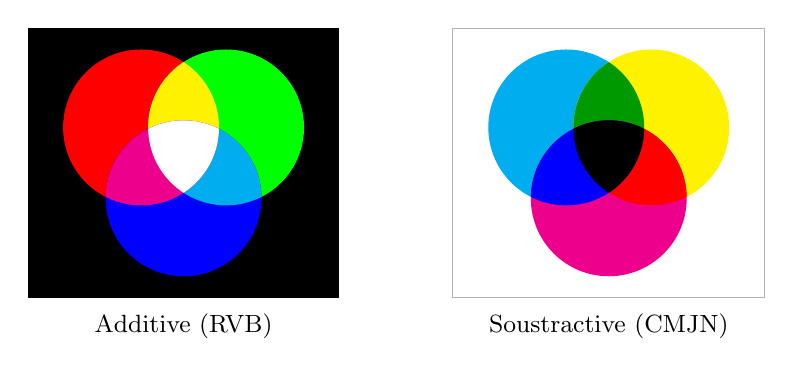
\begin{tikzpicture}[scale=0.9]
% Synthèse additive (RVB) sur fond noir
\begin{scope}
\fill[black] (-2.2,-1.9) rectangle (2.2,1.9);
\fill[red] (-0.6,0.5) circle(1.1);
\fill[green] (0.6,0.5) circle(1.1);
\fill[blue] (0,-0.5) circle(1.1);
\begin{scope}\clip (-0.6,0.5) circle(1.1); \fill[yellow] (0.6,0.5) circle(1.1);\end{scope}
\begin{scope}\clip (0.6,0.5) circle(1.1); \fill[cyan] (0,-0.5) circle(1.1);\end{scope}
\begin{scope}\clip (-0.6,0.5) circle(1.1); \fill[magenta] (0,-0.5) circle(1.1);\end{scope}
\begin{scope}\clip (-0.6,0.5) circle(1.1); \clip (0.6,0.5) circle(1.1); \fill[white] (0,-0.5) circle(1.1);\end{scope}
\node[font=\small] at (0,-2.3) {Additive (RVB)};
\end{scope}
% Synthèse soustractive (CMJN) sur fond blanc
\begin{scope}[xshift=6cm]
\draw[black!30] (-2.2,-1.9) rectangle (2.2,1.9);
\fill[cyan] (-0.6,0.5) circle(1.1);
\fill[yellow] (0.6,0.5) circle(1.1);
\fill[magenta] (0,-0.5) circle(1.1);
\begin{scope}\clip (-0.6,0.5) circle(1.1); \fill[green!60!black] (0.6,0.5) circle(1.1);\end{scope}
\begin{scope}\clip (0.6,0.5) circle(1.1); \fill[red] (0,-0.5) circle(1.1);\end{scope}
\begin{scope}\clip (-0.6,0.5) circle(1.1); \fill[blue] (0,-0.5) circle(1.1);\end{scope}
\begin{scope}\clip (-0.6,0.5) circle(1.1); \clip (0.6,0.5) circle(1.1); \fill[black] (0,-0.5) circle(1.1);\end{scope}
\node[font=\small] at (0,-2.3) {Soustractive (CMJN)};
\end{scope}
\end{tikzpicture}
\caption{À gauche, la lumière additionnée tend vers le blanc. À droite, les encres superposées absorbent la lumière et tendent vers le sombre.}
\end{figure}

\subsubsection{Comment les couleurs sont codées}

Chaque couleur est décrite par trois valeurs, une par canal (rouge, vert, bleu). Dans la plupart des logiciels, chaque valeur va de $0$ à $255$ (8 bits par canal), ce qui donne $256 \times 256 \times 256 = 16\,777\,216$ couleurs possibles.

\begin{table}[h!]
\centering
\begin{tabular}{@{}llll@{}}
\toprule
\textbf{Couleur} & \textbf{R, V, B} & \textbf{Code hexadécimal} & \textbf{Remarque} \\
\midrule
Noir & 0, 0, 0 & \texttt{\#000000} & Aucune lumière \\
Blanc & 255, 255, 255 & \texttt{\#FFFFFF} & Les trois canaux à fond \\
Rouge pur & 255, 0, 0 & \texttt{\#FF0000} & Un seul canal \\
Jaune & 255, 255, 0 & \texttt{\#FFFF00} & Rouge + vert \\
Gris moyen & 128, 128, 128 & \texttt{\#808080} & Trois canaux égaux \\
\bottomrule
\end{tabular}
\caption{Quelques couleurs RVB et leur code hexadécimal.}
\end{table}

\begin{astuce}
Le code hexadécimal est simplement une autre écriture des trois valeurs : \texttt{\#RRVVBB}. Chaque paire de caractères va de \texttt{00} (0) à \texttt{FF} (255). C'est le format utilisé en CSS, et le plus pratique pour échanger une couleur avec un développeur web.
\end{astuce}

\subsubsection{Où utiliser le RVB ?}

Utilise le \terme{RVB} pour tout ce qui sera \emph{vu sur un écran} : sites web, interfaces, réseaux sociaux, présentations, vidéos, applications. Dans \logiciel{Photoshop} comme dans \logiciel{Illustrator}, le mode RVB est le mode de travail naturel pour ces supports.

\subsection{Le système CMJN}

\subsubsection{Définition}

Le système \terme{CMJN} (Cyan, Magenta, Jaune, Noir) est un système de synthèse \terme{soustractive}. Il est utilisé en \emph{impression}. Ici, on ne produit pas de lumière : on dépose de l'encre sur du papier blanc. Chaque encre \emph{absorbe} une partie de la lumière que le papier renvoie. Plus on superpose d'encres, plus la couleur est sombre.

Les trois encres cyan, magenta et jaune, superposées, devraient théoriquement donner du noir. En pratique, les encres réelles donnent plutôt un brun sombre peu net. C'est pourquoi on ajoute une quatrième encre : le \terme{noir}. Dans le sigle CMJN, le N est le noir ; en anglais, on parle de \anglais{CMYK}, où le K vient de \anglais{key} (plaque de référence, qui porte généralement les détails et le texte).

\subsubsection{Comment les couleurs sont codées}

Chaque encre est exprimée en pourcentage, de $0\,\%$ (pas d'encre) à $100\,\%$ (encre pleine). Une couleur CMJN s'écrit donc avec quatre valeurs, par exemple $C=100$, $M=0$, $J=0$, $N=0$ pour un cyan pur.

\begin{defbox}[Le noir riche]
Un noir fait avec $100\,\%$ de noir seul paraît parfois un peu terne sur de grandes surfaces. Les imprimeurs utilisent un \terme{noir riche} : du noir complété par un peu de cyan, de magenta et de jaune. Il est plus profond, mais il ne convient pas aux petits textes, car un léger décalage entre les plaques crée des franges colorées. Pour le texte courant, utilise du noir seul.
\end{defbox}

\subsection{RVB et CMJN : comparaison}

\begin{table}[h!]
\centering
\begin{tabular}{@{}p{3.2cm}p{5.6cm}p{5.6cm}@{}}
\toprule
\textbf{Critère} & \textbf{RVB} & \textbf{CMJN} \\
\midrule
Synthèse & Additive (lumière) & Soustractive (encre) \\
Point de départ & Noir (écran éteint) & Blanc (papier) \\
Mélange total & Blanc & Sombre (noir si on ajoute l'encre noire) \\
Primaires & Rouge, vert, bleu & Cyan, magenta, jaune (+ noir) \\
Unité & Valeurs de 0 à 255 & Pourcentages de 0 à 100 \\
Supports & Écrans, web, vidéo, applications & Imprimés : affiches, flyers, livres, emballages \\
Couleurs possibles & Large, couleurs très vives & Plus restreint, couleurs plus sobres \\
\bottomrule
\end{tabular}
\caption{Comparaison des systèmes RVB et CMJN.}
\end{table}

\begin{erreur}
Il est fréquent de concevoir un visuel en RVB, puis de le convertir en CMJN au dernier moment pour l'impression. Certaines couleurs vives (bleus électriques, verts très saturés, orangés lumineux) n'existent pas en CMJN : elles deviennent plus ternes à la conversion. Si ton projet est destiné à l'impression, travaille en CMJN \emph{dès le départ}, ou au minimum vérifie l'aperçu avant de valider les couleurs.
\end{erreur}

\subsection{Étude de cas : le rouge de Coca-Cola}

Le rouge de la marque Coca-Cola est l'un des exemples les plus connus de couleur devenue identité. On le retrouve sur des canettes, des affiches, des camions, des sites web et des écrans publicitaires. Ce rouge doit pourtant être reproduit sur des supports très différents : lumière émise (écrans), encres sur papier, métal imprimé, tissu, peinture de véhicules.

La leçon pour le designer est la suivante : une couleur de marque ne se définit pas par une seule valeur. Elle est déclinée en plusieurs spécifications (valeurs RVB et hexadécimales pour l'écran, valeurs CMJN pour l'impression, référence Pantone pour les cas où la fidélité est essentielle). C'est ce qu'on trouve dans une \terme{charte graphique}.

\begin{retenir}
\begin{itemize}
  \item Le \terme{RVB} (additif) est fait pour les écrans ; le \terme{CMJN} (soustractif) pour l'impression.
  \item En RVB, chaque canal va de 0 à 255 ; le code hexadécimal est l'écriture \texttt{\#RRVVBB} des mêmes valeurs.
  \item En CMJN, chaque encre va de 0 à 100 \% ; le K (noir) sert aux détails et au texte.
  \item Le RVB couvre plus de couleurs vives que le CMJN : certaines couleurs se ternissent à la conversion.
  \item Choisis le mode colorimétrique \emph{avant} de commencer, selon le support final.
\end{itemize}
\end{retenir}

Nous savons maintenant ce que sont ces deux systèmes. Reste à savoir comment les faire cohabiter sans surprise entre l'écran et le papier : c'est l'objet de la section suivante.

% ============================================================
\section{La gestion des couleurs pour les écrans et l'impression}
% ============================================================

\subsection{Pourquoi la gestion des couleurs est nécessaire}

Tu as sûrement déjà constaté qu'une même photo ne paraît pas identique sur deux téléphones, ou qu'une affiche imprimée est plus terne que sur ton écran. Ce n'est pas un défaut de ton travail : chaque appareil interprète les valeurs numériques à sa manière. Un même triplet RVB, par exemple $(200, 40, 40)$, n'affichera pas exactement la même couleur sur deux écrans différents.

La \terme{gestion des couleurs} (\anglais{color management}) est l'ensemble des méthodes qui permettent d'obtenir des couleurs \emph{prévisibles} d'un appareil à l'autre : écran, imprimante, scanner, appareil photo.

\subsection{Le gamut}

\begin{defbox}[Le gamut]
Le \terme{gamut} (ou \terme{gamme de couleurs}) est l'étendue des couleurs qu'un appareil ou un espace colorimétrique peut reproduire. Une couleur qui ne peut pas être reproduite est dite \terme{hors gamut}.
\end{defbox}

Un écran standard, une imprimante et un appareil photo n'ont pas le même gamut. En général, un écran peut afficher certaines couleurs très vives (bleus et verts lumineux) qu'une impression en quadrichromie ne peut pas reproduire, et inversement certaines nuances d'impression, notamment dans les cyans, sont difficiles à obtenir à l'écran. Quand on convertit d'un espace vers un autre, les couleurs hors gamut sont ramenées vers la couleur reproductible la plus proche.

\subsection{Les profils colorimétriques}

Pour que les couleurs soient interprétées correctement, un fichier peut embarquer un \terme{profil colorimétrique}. C'est un petit fichier de description, normalisé par l'\anglais{International Color Consortium} (\terme{ICC}), qui indique à quel espace appartiennent les valeurs numériques. Sans profil, le logiciel doit deviner.

\begin{table}[h!]
\centering
\begin{tabular}{@{}p{3.2cm}p{5.2cm}p{6cm}@{}}
\toprule
\textbf{Espace / profil} & \textbf{Description} & \textbf{Usage typique} \\
\midrule
sRVB (\anglais{sRGB}) & Espace standard des écrans courants, créé dans les années 1990 & Web, réseaux sociaux, applications : c'est le choix sûr par défaut \\
Adobe RVB (1998) & Gamut plus étendu, surtout dans les verts et cyans & Photographie de qualité, impression photo, écrans compatibles \\
Profils CMJN (par exemple FOGRA39, SWOP) & Décrivent un procédé d'impression et un papier donnés & Impression offset ; le profil dépend du pays, de la machine et du papier \\
\bottomrule
\end{tabular}
\caption{Principaux espaces et profils colorimétriques.}
\end{table}

\begin{astuce}
Pour le web, exporte toujours en \terme{sRVB}. Dans \logiciel{Photoshop}, utilise \emph{Fichier > Exporter > Enregistrer pour le web} (ou convertis en sRVB à l'export) afin que ton image s'affiche de la même manière sur la plupart des navigateurs.
\end{astuce}

\subsection{Les couleurs d'accompagnement : Pantone}

La quadrichromie reproduit les couleurs par mélange de quatre encres. Mais certaines couleurs (métalliques, fluorescentes, ou simplement une couleur de marque que l'on veut parfaitement constante) sont mieux obtenues avec une encre spéciale préparée à l'avance : une \terme{couleur d'accompagnement} (\anglais{spot color}). Le système le plus répandu est le \terme{Pantone} (\anglais{Pantone Matching System}), un nuancier de références numérotées.

Dans \logiciel{Illustrator}, on les retrouve dans les nuanciers (\emph{Fenêtre > Nuanciers}, bibliothèques Pantone). Une couleur d'accompagnement coûte souvent plus cher à l'impression (une encre et une plaque en plus), mais elle garantit la constance de la couleur d'un tirage à l'autre.

\subsection{Étude de cas : une couleur de marque sur tous les supports}

Une marque dont la couleur est reconnaissable (le rouge de Coca-Cola vu plus haut, le jaune d'une enseigne de restauration rapide, le bleu d'un réseau social) doit la maîtriser à tous les niveaux. Sur le réseau social Facebook, le bleu est un élément d'identité très marqué ; il est fréquemment rapporté que son fondateur y est sensible parce qu'il perçoit mal le rouge et le vert, mais l'essentiel pour toi est ailleurs : cette couleur est définie une fois, puis utilisée de manière strictement identique dans l'interface (RVB), sur les supports imprimés (CMJN ou Pantone) et sur les produits dérivés.

Pour un graphiste, cela signifie qu'on ne \og{}choisit\fg{} jamais une couleur de marque à l'œil : on la \emph{retrouve} dans la charte, sous la forme adaptée au support.

\subsection{Flux de travail recommandé}

\begin{enumerate}
  \item \terme{Identifier le support final} : écran, impression, ou les deux.
  \item \terme{Choisir le mode colorimétrique} : RVB (sRVB) pour l'écran, CMJN pour l'impression.
  \item \terme{Régler les profils} : dans \logiciel{Photoshop}, \emph{Édition > Paramètres de couleurs} ; dans \logiciel{Illustrator}, \emph{Fichier > Mode colorimétrique du document}.
  \item \terme{Prévisualiser} : \emph{Affichage > Format d'épreuve} (\logiciel{Photoshop}) permet de simuler le rendu d'impression à l'écran.
  \item \terme{Vérifier les couleurs hors gamut} : \logiciel{Photoshop} peut les signaler par un avertissement.
  \item \terme{Demander une épreuve} (\anglais{proof}) à l'imprimeur pour tout travail important.
\end{enumerate}

\begin{retenir}
\begin{itemize}
  \item Chaque appareil a son propre \terme{gamut} ; la gestion des couleurs vise des résultats prévisibles.
  \item Un \terme{profil ICC} indique l'espace colorimétrique d'un fichier ou d'un appareil.
  \item \terme{sRVB} pour le web ; profil CMJN adapté pour l'impression ; \terme{Pantone} quand la couleur doit être constante.
  \item Prévisualise toujours le rendu d'impression à l'écran, et demande une épreuve pour les travaux importants.
\end{itemize}
\end{retenir}

Même avec une bonne gestion des couleurs, il reste des pièges très répandus dans l'usage de la couleur. C'est ce que nous allons passer en revue pour finir.

% ============================================================
\section{Les erreurs courantes dans l'utilisation des couleurs}
% ============================================================

\subsection{Erreurs de conception}

\subsubsection{Trop de couleurs}

Utiliser sept ou huit couleurs sans hiérarchie fatigue l'œil et brouille le message. Une palette de trois à cinq couleurs, avec des neutres, suffit presque toujours.

\subsubsection{Contraste insuffisant}

Du texte gris clair sur fond blanc, ou du texte jaune sur fond blanc, devient difficile à lire. Le contraste entre le texte et le fond doit être suffisant, en particulier pour les petits corps et pour les personnes malvoyantes. Les recommandations d'accessibilité web (\anglais{WCAG}) donnent des ratios de contraste minimaux à respecter.

\subsubsection{Associations qui vibrent}

Placer des couleurs très saturées et de même luminosité côte à côte (par exemple un rouge vif sur un vert vif) crée un effet de vibration désagréable.

\subsubsection{Couleur comme seule information}

Un graphique ou une interface qui distingue ses éléments \emph{uniquement} par la couleur est inutilisable pour les personnes daltoniennes. Ajoute une seconde information : une forme, un motif, une étiquette, une icône.

\begin{erreur}
Une partie importante de la population, surtout masculine, est atteinte de daltonisme (confusion entre certains rouges et verts, le plus souvent). Ne signale jamais un état (erreur / succès, positif / négatif) uniquement par du rouge et du vert.
\end{erreur}

\subsection{Erreurs de signification}

Ignorer le public et le contexte culturel conduit à des contresens. Le cas du deuil le montre bien : dans de nombreux pays occidentaux, le noir est associé au deuil, alors que dans plusieurs pays d'Asie (la Chine, l'Inde, par exemple), c'est le blanc qui est traditionnellement associé aux funérailles. Un visuel conçu pour une audience internationale doit tenir compte de ces écarts.

\begin{table}[h!]
\centering
\begin{tabular}{@{}p{2.4cm}p{6cm}p{6cm}@{}}
\toprule
\textbf{Couleur} & \textbf{Association fréquente} & \textbf{Nuance culturelle} \\
\midrule
Blanc & Pureté, propreté (contexte occidental) & Associé au deuil dans plusieurs pays d'Asie \\
Noir & Élégance, luxe ; deuil en Occident & Autres connotations selon les cultures \\
Rouge & Passion, danger, urgence & Associé à la chance et à la fête en Chine \\
\bottomrule
\end{tabular}
\caption{Quelques écarts d'interprétation d'une culture à l'autre.}
\end{table}

\subsection{Erreurs techniques}

\begin{itemize}
  \item \terme{Mauvais mode colorimétrique} : fichier RVB envoyé à l'imprimeur sans conversion contrôlée.
  \item \terme{Absence de profil} : les couleurs s'affichent différemment selon le logiciel.
  \item \terme{Couleurs hors gamut ignorées} : un bleu électrique devient terne à l'impression.
  \item \terme{Écran non calibré} : tu juges les couleurs sur un écran trop clair, trop chaud ou trop contrasté.
  \item \terme{Noir mal défini} : petit texte en noir riche (franges colorées) ou grand aplat en noir seul (aspect terne).
  \item \terme{Ne pas faire d'épreuve} : on découvre le résultat à la livraison des 5\,000 exemplaires.
\end{itemize}

\subsection{Étude de cas : le rouge et le jaune d'une enseigne de restauration rapide}

Beaucoup d'enseignes de restauration rapide associent le rouge et le jaune dans leur identité (c'est le cas bien connu de McDonald's). Cette association est souvent expliquée par ses effets : le rouge attire l'œil et est associé à l'énergie, le jaune à la visibilité et à la bonne humeur. Pour ce chapitre, retiens l'enseignement de méthode : ces deux couleurs fortes, très contrastées avec les neutres, sont employées avec \emph{une hiérarchie claire} (une dominante, un accent) et de façon constante sur tous les supports. L'efficacité vient de la cohérence, pas du nombre de couleurs.

\subsection{Liste de contrôle}

\begin{table}[h!]
\centering
\begin{tabular}{@{}p{9cm}p{5cm}@{}}
\toprule
\textbf{Question à te poser} & \textbf{Section concernée} \\
\midrule
La palette tient-elle en cinq couleurs ou moins, avec des neutres ? & Palette \\
Le texte est-il lisible sur son fond (contraste) ? & Teinte, saturation, luminosité \\
Le message reste-t-il compréhensible pour un daltonien ? & Erreurs de conception \\
Les couleurs conviennent-elles au public et à sa culture ? & Psychologie des couleurs \\
Le mode (RVB / CMJN) correspond-il au support ? & RVB et CMJN \\
Ai-je prévisualisé ou fait une épreuve ? & Gestion des couleurs \\
\bottomrule
\end{tabular}
\caption{Liste de contrôle avant de valider un travail en couleur.}
\end{table}

\begin{retenir}
\begin{itemize}
  \item Limite le nombre de couleurs, vérifie le contraste et n'utilise jamais la couleur comme seule information.
  \item Tiens compte du contexte culturel du public visé.
  \item Évite les erreurs techniques : bon mode colorimétrique, profils, hors gamut, écran calibré, épreuve.
\end{itemize}
\end{retenir}

% ============================================================
\section*{Exercices pratiques}
\addcontentsline{toc}{section}{Exercices pratiques}
% ============================================================

\subsubsection*{Exercice 1 --- Palette à partir d'une photo (\logiciel{Photoshop})}

Choisis une photo (paysage, objet, portrait). Avec l'outil \emph{Pipette}, prélève cinq couleurs : une dominante, deux secondaires, un accent et un neutre. Crée un nouveau document de $1200 \times 400$ pixels en mode RVB et dispose les cinq couleurs sous forme de cinq rectangles, avec leur code hexadécimal écrit dessous.

\noindent\textbf{Critère de réussite :} la palette est cohérente (on devine la photo d'origine), les cinq codes hexadécimaux sont lisibles, et on identifie sans hésiter la dominante et l'accent.

\subsubsection*{Exercice 2 --- Harmonies avec Adobe Color et \logiciel{Illustrator}}

Sur \emph{Adobe Color}, construis successivement une harmonie analogue, une harmonie complémentaire et une harmonie triadique à partir de la même teinte de base. Reporte chacune dans \logiciel{Illustrator} sous forme de cinq pastilles (cercles) et nomme les nuanciers.

\noindent\textbf{Critère de réussite :} trois nuanciers enregistrés, chacun de cinq couleurs, dont on peut dire en une phrase l'effet produit (douceur, contraste, équilibre).

\subsubsection*{Exercice 3 --- Du RVB au CMJN (\logiciel{Photoshop} et \logiciel{Illustrator})}

Crée une affiche A5 de ton choix en RVB avec au moins une couleur très vive (bleu électrique ou vert saturé). Convertis-la en CMJN (\emph{Image > Mode > Couleurs CMJN}) et compare avant et après, avec \emph{Affichage > Format d'épreuve}. Dans un court commentaire, note quelles couleurs ont changé le plus et corrige-les manuellement.

\noindent\textbf{Critère de réussite :} deux versions (RVB et CMJN) présentées côte à côte, un commentaire identifiant au moins deux couleurs modifiées, et une version CMJN finale dont les couleurs te semblent équilibrées.

% ============================================================
\section*{Conclusion du chapitre}
\addcontentsline{toc}{section}{Conclusion du chapitre}
% ============================================================

Nous voici au terme du chapitre 3. Nous avons étudié la couleur sous ses principaux aspects :

\begin{itemize}
    \item \terme{Définition et rôle} : la couleur attire l'attention, hiérarchise, identifie, émeut, signifie et organise.
    \item \terme{Cercle chromatique} : primaires, secondaires, tertiaires et leurs relations.
    \item \terme{Chaud et froid} : la température des couleurs et ses effets.
    \item \terme{Teinte, saturation, luminosité} : les trois dimensions d'une couleur.
    \item \terme{Harmonies} : complémentaires, analogues, triadiques, tétradiques.
    \item \terme{Psychologie et culture} : des associations utiles mais relatives.
    \item \terme{Palette} : un ensemble limité, hiérarchisé et testé.
    \item \terme{RVB et CMJN} : lumière pour l'écran, encre pour l'impression.
    \item \terme{Gestion des couleurs} : gamut, profils, Pantone, épreuves.
    \item \terme{Erreurs courantes} : trop de couleurs, contraste, daltonisme, culture, technique.
\end{itemize}

La couleur est un outil puissant, mais elle ne travaille jamais seule : elle s'appuie sur la composition que nous avons vue, et elle s'associe à la typographie, dont nous allons maintenant explorer les principes.

\vspace{1em}

\begin{center}
\textbf{Prochain chapitre : Chapitre 4 --- Typographie et communication visuelle.}
\end{center}
